%%%%%%%%%%%%%%%%%%%%%%%%%
% Load Preample         %
%%%%%%%%%%%%%%%%%%%%%%%%%

\documentclass[a4, danish]{article}
%%%%%%%%%%%%%%%%%%%%%%%%%%%%%%%%%%
% Settings for document (danish) %
%%%%%%%%%%%%%%%%%%%%%%%%%%%%%%%%%%

% Input common definition
%%%%%%%%%%%%%%%%%%%%%%%%%%%%%%%%
%    Papersize and encoding    %
%%%%%%%%%%%%%%%%%%%%%%%%%%%%%%%%

% Size of margins can be changed here in the outcommented version!
%\usepackage[a4paper, total={6in, 8in}]{geometry}	%total={width, height}
\usepackage[a4paper]{geometry}

% Basics: font, codec etc.
\usepackage[utf8]{inputenc}						% encoding: utf-8 (nordic letters)
\usepackage[T1]{fontenc}						% use 8-bit encoded fonts
\renewcommand{\sfdefault}{phv}					% changes the default font

%\usepackage[parfill]{parskip}      %Instead of indenting on a newline adds whitespace



%%%%%%%%%%%%%%%%%%%%%%%%%%%%%%%%
%      Tables and figures      %
%%%%%%%%%%%%%%%%%%%%%%%%%%%%%%%%

\usepackage{tabularx,booktabs,authblk}		    % various basic stuff for tables and more

% Figures and captions
\usepackage{caption}							% create captions for figures
\usepackage{subfig}								% create subfigures of a figure
%\usepackage{subcaption}					% create captions for subfigures
                                  %     currently off, due to conflicts

\usepackage{wrapfig}							% letting figures be in text

\usepackage{rotating}             % let any environment be rotated (figures sideways)
                                  %     \begin{sideways} or \begin{turn}{30}



%%%%%%%%%%%%%%%%%%%%%%%%%%%%%%%%%%%%
%           Variables              %
%%%%%%%%%%%%%%%%%%%%%%%%%%%%%%%%%%%%
\usepackage{pgfkeys}			%Initialize the variable key-value parirs

\newcommand{\setvalue}[1]{\pgfkeys{/variables/#1}}
\newcommand{\getvalue}[1]{\pgfkeysvalueof{/variables/#1}}
\newcommand{\declare}[1]{%
 \pgfkeys{
  /variables/#1.is family,
  /variables/#1.unknown/.style = {\pgfkeyscurrentpath/\pgfkeyscurrentname/.initial = ##1}
 }%
}

\declare{}



%%%%%%%%%%%%%%%%%%%%%%%%%%%%%%%%
%      LaTeX Programming       %
%%%%%%%%%%%%%%%%%%%%%%%%%%%%%%%%

\usepackage{xparse}								% Scanning arguments
\usepackage{xifthen}							% Conditionals
\usepackage{xstring}                            % String functions
\usepackage{calc}								% Calculations



%%%%%%%%%%%%%%%%%%%%%%%%%%%%%%%%
%          Hypermedia          %
%%%%%%%%%%%%%%%%%%%%%%%%%%%%%%%%

\usepackage{url, hyperref}							% \url{link} and \href{link}{replacing text}

%Macros taken from the preamble of the MatFysTutor LaTeX Guide.
\newcommand*{\http}[1]{\href{http://#1}{#1}}		% macro for http links: \http{www.matfystutor.dk}
\newcommand*{\mailto}[1]{\href{mailto:#1}{#1}}		% macro for mails: \mailto{email@email.com}

%%%%%%%%%%%%%%%%%%%%%%%%%%%%%%%%
%         Stylization          %
%%%%%%%%%%%%%%%%%%%%%%%%%%%%%%%%

% Headers og footers
\usepackage{lastpage}                           % \lastpage command for numbers of pages
\usepackage{fancyhdr}                           % create cool headers and footers
\pagestyle{fancy}                               % who doesn't want their page to be fancy?

% Use of columns
\usepackage{multicol}

% Quotations
% "danish" or "british"
\usepackage[danish=guillemets]{csquotes}    	% two styles: "quotes" or >>guillemets<<
%\MakeAutoQuote{»}{«}                       	% decomment for easy macro
%\MakeAutoQuote*{›}{‹}                      	% decomment for even easier macros

% Like a paragraph, but adds also a linebreak after. (Also is not recorded on labelling)
\newcommand{\lbparagraph}[1]{\vspace{0.3em} \noindent \textbf{#1}\\ \noindent}

%%%%%%%%%%%%%%%%%%%%%%%%%%%%%%%%
%             Math             %
%%%%%%%%%%%%%%%%%%%%%%%%%%%%%%%%
%\newcommand{\hmmax}{0}								% minimizes the amount of bold families
%\newcommand{\bmmax}{1}								% this allows for more math families

% various basic stuff
\usepackage{mathtools, amsmath}
\allowdisplaybreaks                                 % allow pagebreaks in align* ?

% Various symbol packages
\usepackage{amssymb}
\usepackage[utopia]{mathdesign}					    % full overwrite of the font system
\usepackage{stmaryrd}								% even more symbols

\DeclareMathAlphabet{\mathpzc}{OT1}{pzc}{m}{it}     % \mathpzc a less pompous curly typeset

% Math shortcuts
\renewcommand{\d}{\, \mathrm{d}}                    % \d = differential d with a bit of spacing
\newcommand{\e}{\mathrm{e}}                         % \e = eulers number
\newcommand{\R}{\mathbb{R}}                         % \R = Real numbers
\newcommand{\N}{\mathbb{N}}                         % \N = Natural numbers
\newcommand{\C}{\mathbb{C}}                         % \C = Complex numbers
\newcommand{\Q}{\mathbb{Q}}                         % \Q = Rational numbers
\newcommand{\F}{\mathbb{F}}							% \F

\newcommand{\abs}[1]{\left\lvert #1 \right\rvert}			% \abs{arg}		absolute/modulo of value
\newcommand{\norm}[1]{\left\lVert #1 \right\rVert}			% \norm{arg}	norm of a value
\newcommand{\ceil}[1]{\left\lceil #1 \right\rceil}			% \ceil{arg}	ceiling of a value
\newcommand{\floor}[1]{\left\lfloor #1 \right\rfloor}		% \floor{arg}	floor of a value
\newcommand{\inprod}[2]{\left\langle #1 , #2 \right\rangle}	% \inprod{arg}	inner product

\newcounter{i}

\DeclareDocumentCommand \seq { g g g g } {			% \seq{x}{i}{j}{s}
	\setcounter{i}{0}								% x_i, x_i+s, ... x_j
	\IfValueT {#2} { \addtocounter{i}{#2} }
	\IfValueTF {#1}
		{#1}
		{x}
	_{ \arabic{i} },
	\IfValueTF {#4} 
		{\addtocounter{i}{#4}}
		{\addtocounter{i}{1}}
	\IfValueTF {#1} 
		{#1}
		{x} 
	_{ \arabic{i} },
	\dots
	\IfValueTF {#3}
		{ , #1_{#3} }
		{}
}

\DeclareDocumentCommand \ero { g g } {				% \ero {x, y}
	\begin{array}{c}								%	x
		\IfValueTF{#1}								%	~
			{_{#1}}									%	y
			{\phantom{\sim}}
	\\
		\sim
	\\
		\IfValueTF{#2}
			{^{#2}}
			{\phantom{\sim}}
	\end{array}
}

\DeclareDocumentCommand \set { m g }{ 				% \sets{X}{C}
	 \left\lbrace									% {X | C}
	 	#1 \IfValueT {#2} { \ | \  #2 }
	 \right\rbrace
}

\makeatletter										% adds vertical lines to matrices
\renewcommand*\env@matrix[1][*\c@MaxMatrixCols c]{
  \hskip -\arraycolsep
  \let\@ifnextchar\new@ifnextchar
  \array{#1}}
\makeatother

%%%%%%%%%%%%%%%%%%%%%%%%%%%%%%%%
%      Logic and proofs        %
%%%%%%%%%%%%%%%%%%%%%%%%%%%%%%%%

% Proofs
\usepackage{amsthm}								% Theorem package
\theoremstyle{definition}						% plain, definition, remark
%\swapnumbers									% If you want to have the number first

% Logic packages
\usepackage{lplfitch}						% fitch style proofs

%\usepackage{logicproof}					% alternative package, resembling the dBerLog book
%\setlength\subproofhorizspace{2em}			% Indent for subproofs. Changed for fresh variables



%%%%%%%%%%%%%%%%%%%%%%%%%%%%%%%%
%      Color and presets       %
%%%%%%%%%%%%%%%%%%%%%%%%%%%%%%%%

%\usepackage{xcolor}							% basic xcolor package
\usepackage[table,xcdraw]{xcolor}				% xcolor package with support for tables
\definecolor{lstComment}{rgb}{0.45,0.45,0.45}	% code: comments (Grey)
\definecolor{lstKey}{rgb}{0.13,0.21,1}			% code: primary keywords (Blue)
\definecolor{lstKey2}{rgb}{1,0.666667,0.13726}  % code: secondary keywords (Day[9] Orange)
\definecolor{lstString}{rgb}{0.1,0.65,0.1}		% code: strings (Green)
\definecolor{lstBase}{rgb}{0.0,0.0,0.0}			% code: base (Black)



%%%%%%%%%%%%%%%%%%%%%%%%%%%%%%%%
%            Tikz              %
%%%%%%%%%%%%%%%%%%%%%%%%%%%%%%%%

\usepackage{tikz}								% import basepackage
\usetikzlibrary{calc}							% Coordinate calcuations
\usetikzlibrary{positioning}                    % Relative positioning
\usetikzlibrary{shapes}                         % Defining nodeshapes and more (isa for E/R)

% Simple tree macro with compability to tikz
\usepackage{tikz-qtree}							% import simple tree macro
\usetikzlibrary{arrows}                         % arrows for trees

% Tikz settings for red-black trees
\tikzset{
  treenode/.style = {align=center, inner sep=0pt, text centered,
    font=\sffamily},
  arn_b/.style = {treenode, circle, white, font=\sffamily\bfseries, draw=black,
    fill=black, text width=1.5em},              % black node
  arn_r/.style = {treenode, circle, white, font=\sffamily\bfseries, draw=red,
    fill=red, text width=1.5em},              % red node
  arn_x/.style = {treenode, rectangle, draw=black, fill=black,
    minimum width=0.5em, minimum height=0.5em}  % nil node
}

% Tikz Automota for Turing Machines
\usetikzlibrary{automata}

% Tikz E/R diagram
\usetikzlibrary{er}

% Graphics and plots
\usepackage{graphicx}							% import basepackage for graphs
\usepackage{pgfplots}							% import pgfplots
\usepgfplotslibrary{fillbetween}				% add fillBetween command
\pgfplotsset{compat=1.10}						% choose version of pgfplots

% Macro for circle with symbol inside.
\newcommand*\circled[1]{ \tikz[baseline=(C.base)]\node[draw,circle,inner sep=0.5pt](C) {#1};\!}



%%%%%%%%%%%%%%%%%%%%%%%%%%%%%%%%
%            Code              %
%%%%%%%%%%%%%%%%%%%%%%%%%%%%%%%%
\newcommand{\code}[1]{{\sf #1}}					% \code{X} writes X in a code-appropriate font




%%%%%%%%%%%%%%%%%%%%%%%%%%%%%%%%
%         lstlisting           %
%%%%%%%%%%%%%%%%%%%%%%%%%%%%%%%%

% Import lstlistings - beautiful sourcecode!
\usepackage{listings}


% Custom language definitions
% Definition of Pseudocode
\lstdefinelanguage{pseudocode}{
  keywords=[1]{
  	     by, by, do, downto, else, error, for, if, repeat, return, to, until, while, while
  	},								    		% list of keywords, first and last are not used
  keywords=[2]{
        and, and, or, NIL, NIL
  }
  sensitive=false,								% keywords are not case-sensitive
  morecomment=[l]{//},							% l is for line comment
  morecomment=[s]{/*}{*/},						% s is for start and end delimiter
  morestring=[b]"								% strings are enclosed in double quotes
}


% Settings for lstlistings
\lstset{language=pseudocode,					% choose language
  columns=flexible,								% let the box align to the width of the page
    literate={æ}{{\ae}}1{ø}{{\o}}1{å}{{\aa}}1	% allow æ, ø and å in code
           {Æ}{{\AE}}1{Ø}{{\O}}1{Å}{{\AA}}1,	% 	(this change was taken from the preamble of the MatFysTutor LaTeX Guide)
  breaklines=true,								% automatically break lines
  breakatwhitespace=true,						% automatically break should there only be white space.
  numbers=left,									% numbering: none, left, right
  numbersep=5pt,								% distance between linenumbers and code
  numberstyle=\color{lstComment},				% change style of numbering - currently grey.
  stepnumber=1,									% step between to line-numbers. 1 = each line is numbered
  showspaces=false,								% show spaces everywhere - adding particular underscores
  showstringspaces=false,						% underline spaces within strings only.
  showtabs=false,								% show tabs within strings adding particular underscores.
  escapeinside={*@}{@*},                		% if you want to add LaTeX within your code
  basicstyle=\ttfamily \color{lstBase},			% set basic color
  commentstyle=\color{lstComment},				% set color of comments
  keywordstyle=[1]\color{lstKey},				% set color of primary keywords
  keywordstyle=[2]\color{lstKey2},				% set color of secondary keywords
  stringstyle=\color{lstString},				% set color of strings
}

% lstlisting - Put it beautifully in the middle
\lstset{xleftmargin= .1\textwidth ,     							% leftmargin being 10% of the current width
  xrightmargin= .1\textwidth,           							% right margin also 10%
  frame=bottomline                      							% Draw a line on the bottom of the surrounding box
}

% lstlisting header
\DeclareCaptionFont{white}{\color{white}}                                       % fontstyle of caption
\DeclareCaptionFormat{listing}{\colorbox{gray}{\parbox{\linewidth}{#1#2#3}}}    % create nice grey boxes for captions
\captionsetup[lstlisting]{format=listing,labelfont=white,textfont=white}        % apply settings to listing


%%%%%%%%%%%%%%%%%%%%%%%%%%%%%%%%%%%%
%      Title and information       %
%%%%%%%%%%%%%%%%%%%%%%%%%%%%%%%%%%%%
\setvalue{title = }
\setvalue{subtitle = }

\DeclareDocumentCommand \settitle { m g }{ 				% \setTitle{title}{subtitle}
	 \setvalue{title = #1}
	 \IfValueTF {#2} { \setvalue{subtitle = #2} \title{\huge \getvalue{title} \\ \large \getvalue{subtitle}}}
	 				 { \title{\huge \getvalue{title}} }
}

\DeclareDocumentCommand \addauth { m g g }{ 			% \addAuth{name}{email}{id}
     \IfValueT {#3} {		%Set the id text as desired on the top left
	 	\setvalue{id = #3}
	 }
     \pgfkeysifdefined{/variables/name}{
         \setvalue{id = \, et al}
     }{
         \setvalue{name = #1}
     }	 
	 \author{#1}
	 \IfValueT {#2} {
	    \pgfkeysifdefined{/variables/email}{
	        % Do Nothing
	    }{
	 	    \setvalue{email = #2}
	 	}
	 	\affil{\protect\href{mailto:#2}{#2}}
	 }
}

\settitle{Keep Calm and \textbackslash settitle}

\date{\today}

\setvalue{of = of}

\lhead{\protect\href{\getvalue{email}}{\getvalue{name}\getvalue{id}} \\ \getvalue{title}}
\chead{}
\rhead{\thepage\ \getvalue{of} \pageref{LastPage} \\ \nouppercase{\leftmark}}

%\lfoot{}
%\cfoot{}
%\rfoot{}


%%%%%%%%%%%%%%%%%%%%%%%%%%%%%%%%
%   Encoding and hyphenation   %
%%%%%%%%%%%%%%%%%%%%%%%%%%%%%%%%
% Basics: font, codec etc.
\usepackage[danish]{babel}                        % babel is for hyphenation and other goodies
\renewcommand{\danishhyphenmins}{22}              % even better danish hyphenation!

% .bib danish redefinition for author in title
\renewcommand\Authand{ og }
\renewcommand\Authands{, og }
\renewcommand\Affilfont{\small}



%%%%%%%%%%%%%%%%%%%%%%%%%%%%%%%%
%         lstlisting           %
%%%%%%%%%%%%%%%%%%%%%%%%%%%%%%%%

% lstlisting language redefinitions
\renewcommand{\lstlistingname}{Kode}                                            % for one block of code alone
\renewcommand{\lstlistlistingname}{Liste af \lstlistingname r}                  % for more pieces of code in one



%%%%%%%%%%%%%%%%%%%%%%%%%%%%%%%%
%      Logic and proofs        %
%%%%%%%%%%%%%%%%%%%%%%%%%%%%%%%%
% Theorem environments
\newtheorem{theorem}{Sætning}[section]
\newtheorem{lemma}[theorem]{Lemma}
\newtheorem{proposition}[theorem]{Proposition}
\newtheorem{corollary}[theorem]{Korollar}
\newtheorem{definition}[theorem]{Definition}
\newtheorem{conjecture}[theorem]{Formodning}
\renewcommand*{\proofname}{Bevis}


%%%%%%%%%%%%%%%%%%%%%%%%%%%%%%%%
%      Example environment     %
%%%%%%%%%%%%%%%%%%%%%%%%%%%%%%%%
\newtheorem{example}[theorem]{Eksempel}
\newtheorem{problem}[theorem]{Problem}

%%%%%%%%%%%%%%%%%%%%%%%%%
% Document starts here! %
%%%%%%%%%%%%%%%%%%%%%%%%%

\begin{document}

% Define title and more on frontpage
    \title{\huge Title \\ \large Subtitle}
    
    \author{Steffan C. S. Jørgensen}
    \affil{
        \protect\href{mailto:201505832@post.au.dk}{201505832@post.au.dk}
    }
    
    \date{\today}
    
    \lhead{\protect\href{mailto:201505832@post.au.dk}{Steffan Sølvsten, 201505832}}
    \chead{}
    \rhead{\@currentlabelname\ | \thepage\ of \pageref{LastPage}}

    %\lfoot{}
    %\cfoot{}
    %\rfoot{}
\maketitle

\begin{abstract}
\noindent Lorem ipsum dolor sit amet, consectetur adipiscing elit, sed do eiusmod tempor incididunt ut labore et dolore magna aliqua.
\end{abstract}

%En indholdsfortegnelse kan nemt laves med \tableofcontents funktionen
\tableofcontents

\newpage
\section{Matematik} \label{sec:math}
Mest basalt kan man bruge \emph{equation} til at skrive matematik på en linje eller matematik i teksten skrives med \$ x\_0 \$ = $x_0$.

Skal man skrive matematik over flere linjer, så er det bedre at bruge \emph{align} eller ved mere komplicerede ting \emph{alignat}. Det følgende eksempel er \emph{alignat}, der gør det muligt at justere efter flere ting: Her både pilene til venstre og lighedstegnene.

\begin{alignat}{2}
&& cos x &= cos x * cos y \label{alignatL1}
\\ \ArrowBetweenLines
&& 0 &= cos x * cos y - cos x \label{alignatL2}
\\ \ArrowBetweenLines
&& 0 &= cos x (cos y - 1) \label{alignatL3}
\end{alignat}

Her er desuden en reference til linje \ref{alignatL2}.

\subsection{Matricer}
Med \emph{pmatrix} kan man lave matricer
\begin{equation*}
	\begin{pmatrix}
		v_1 * v_1 & v_1 * v_2 & \dots & v_1 * v_n
\\		v_2 * v_1 & \ddots & & \vdots
\\		\vdots & & \ddots & \vdots
\\		v_n * v_1 & \dots & \dots & v_n * v_n
	\end{pmatrix}
\end{equation*}


\section{Beviser}
Der findes mange forskellige pakker for at lave beviser, hvor efter længere søgen har jeg til sidst valgt at bruge \emph{lplfitch} pakken, da fitch-style beviser synes at være den mest anvendte metode for at danne beviser indenfor logik. For syntaksen skal man dog holde tungen meget lige i munden
\begin{center}
    \fitchprf{\pline[1.]{antagelse}}{
        \pline[2.]{konklussion}
    \\
    	\subproof{\pline[3.]{antagelse}}{
    		\pline[4.]{konklussion}[begrundelse]
    	\\
    		\pline[5.]{konklussion}
    	}
    	\pline[6.]{konklussion}
    }
\end{center}

Denne pakke indeholder tilsyneladende ikke meget syntaktisk sukker i forhold til andre, hvorfor brug af dokumentation for at kende genveje muligvis er nødvendigt, dog er de alle på formen: $"l" + type + "i/e"$. Argumentation gøres også ved genveje. Hver linje er skrevet på formen
\begin{equation*}
    pline[hline number i]\{hformulai\}[hjustificationi]
\end{equation*}

\newpage
Bemærk, at normalt i fitch-style bliver der ikke skrevet assumption eller premise, men det markeres i stedet med en vandret streg. Du kan dog nemt skrive det selv, hvis ønsket. Hermed vil beviset $1.2.1$ c fra TØ skrives som
\begin{center}
    \fitchprf{\pline[1.]{(p \land q) \land r}[\textbf{Premise}]}{
    	\pline[2.]{r}[\lande{1}]
    \\
        \pline[3.]{p \land q}[\lande{1}]
    \\
        \pline[4.]{p}[\lande{3}]
    \\
        \pline[5.]{q}[\lande{3}]
    \\
        \pline[6.]{q \land r}[\landi{2, 5}]
    \\
        \pline[7.]{p \land (q \land r)}[\landi{4, 6}]
    }
\end{center}

\section{Figurer og grafer}
Følgende er en figur indeholder et billede. Figurens label er \ref{FigExample}.

\begin{figure}[htbp] %htbp forces the figure into the text.
    \centering
    \includegraphics[width=10em]{picture.png}
    \caption{Et billede}
    \label{FigExample}
\end{figure}

Figurer behøver dog ikke at indeholdet et billede og i stedet for \emph{includegraphics} kan alt muligt andet indsættes. Bare eksperimenter en smule.

\begin{wrapfigure}[10]{r}{15em}
	\centering
	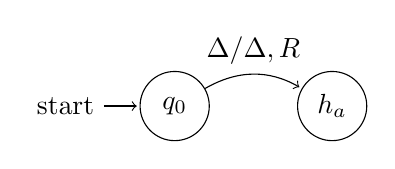
\begin{tikzpicture}[shorten >= 1, node distance = 2cm, on grid, auto]
	\node[state, initial] (0) {$q_0$};
	\node[state] (h) [right=of 0] {$h_a$};
	\path[->]
		(0) edge [bend left] node {$\Delta / \Delta , R$} (h);
	\end{tikzpicture}
	\caption{Transition diagram of a small Turing machine}
	\label{fig:TM2}
\end{wrapfigure}
Hvis man gerne vil have figurer ved siden af sin tekst, så kan der bruges en \emph{wrapfigure} i stedet for en normal \emph{figure}. Skriv teksten på den linje, som du ønsker at billedet starter på. Den første variabel er antallet af linjer, hvor kassen skal være høj. Den anden variable er venstre eller højre og til sidst er der bredden af figuren.

\newpage
\section{Grafer}
Her er en graf fra vores første Calculus Opgave, Tak Rasmus. \cite{rasmus}

\begin{center}
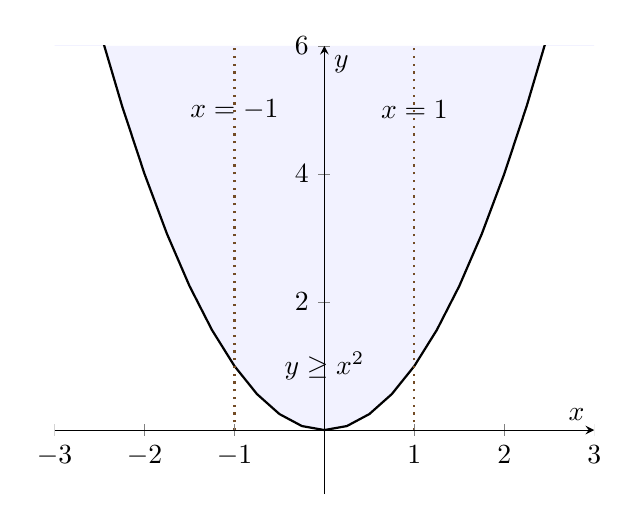
\begin{tikzpicture}
\begin{axis}[
    xmin=-3, xmax=3,
    ymin=-1, ymax=6,
    xlabel={$x$},ylabel={$y$},
    axis lines=center,
    axis on top=true,
    ]
    %Graf x^2
    \addplot [name path=f, domain=-3:3,black, thick] {x^2};
    %Øverste kant for fill
    \path[name path=axis] (axis cs:-3,6) -- (axis cs:3,6);
    %Indstillinger for fill
    \addplot [
        thick,
        color=blue,
        fill=blue, 
        fill opacity=0.05
    ]
    %Start af fill
    fill between[
        of=f and axis,
    ];
    
    %Tegner lodrette streger
    \addplot+[ycomb,dotted,thick,no marks] table[x=x,y expr=6] {
    x
    -1
    1
    };
    
    %Tilføjer tekst
    \node [] at (axis cs:  -1, 5) {$x=-1$};
    \node [] at (axis cs:  1, 5) {$x=1$};
    \node at (axis cs:  0, 1) {$y\geq x^2$};    
\end{axis}
\end{tikzpicture}
\end{center}

\noindent Dette kan også indsættes i en figur i stedet for linjen \emph{includegrapics}, så der er caption og referencer.

\section{Kode}
Følgende er lidt sourcecode til noget ubrugelig Java. hvis man ikke vil have \emph{Kode X:}, så kan man bruge \emph{title} frem for \emph{caption}. Dette får dog \emph{label} til at gå i stykker, så hvis man generelt vil have det fjernet, så ændre i definitionen øverst. Følgende kode har label \ref{lst:Example}

\begin{lstlisting} [label={lst:Example},
	caption={Jeg er en caption}]
//This is a comment, nordic letters are not supported
public static String example(int n) {
	return "You wrote: "+n;
}
\end{lstlisting}

Skal sproget sættes til noget andet end i begyndelsen, så gøres dette også meget nemt. I følgende pseudokode bruges også escape character parrene *@ og @* for at indsætte \LaTeX\ matematik.

\begin{lstlisting}[language=pseudocode,
                firstnumber=1,
                caption={The algorithm \emph{linear exponentiation}},
                label={lst:algorithm}]
*@ \textbf{Algorithm: Linear Exponentiation} @*(x,p)
 Input     : *@ $p \geq 0$ @*
 Output    : *@ $r = x^p$ @*
 Method    : *@ $r \leftarrow 1$ @*
             *@ $q \leftarrow p$ @*
              {I} while *@ $q > 0$ @* do
                    *@ $r \leftarrow r * x$ @*
                    *@ $q \leftarrow q - 1$ @*
\end{lstlisting}

\newpage
\section{Træer}
Med qtree er det meget hurtigt at tegne træer. Bemærk dog, at du skal have et mellemrum mellem indholdet og den lukkende parantes.

\begin{figure}[htbp]
    \centering
    \Tree [.rod [.{rod for et subtræ}
				blad
				blad ]
			blad ]
    \caption{Et træ}
    \label{fig:tree1}
\end{figure}

Skal træerne være lidt mere komplekse eller smukke, så kan man bruge tikz, som allerede er sat op i starten til at lave rød-sorte træer.

\begin{figure}[htbp]
    \centering
    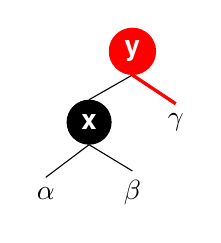
\begin{tikzpicture}[baseline={(current bounding box.center)},-,>=stealth',level/.style={sibling distance = 1.1cm, level distance = 0.9cm}]
            \node [arn_r] {y}
                child{ node [arn_b] {x} 
                    child{ node {$\alpha$} }
                    child{ node {$\beta$} }                            
                }
                child[style={edge from parent/.style={red,very thick,draw}}]
                    { node {$\gamma$} }
            ;
    \end{tikzpicture}
    \caption{Et pænere træ}
    \label{fig:tree2}
\end{figure}

\section{Automater}
Ved brug af en udvidelse til Tikz er dannelsen af automater meget enkelt. Det eneste besværlige er de længere streger, som transitionen fra (C) til (A) over 1, hvilket her i koden er kommenteret, idet det også er muligt at bestemme vinklen af kanterne.
\begin{figure}[htbp]
	\centering
	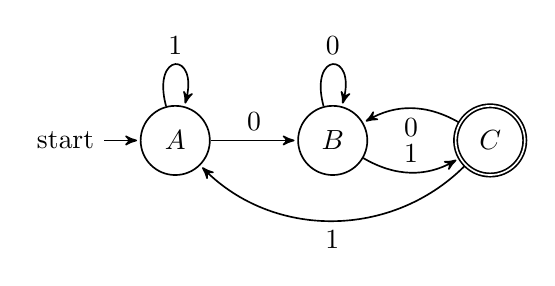
\begin{tikzpicture}[>=stealth', semithick,                                  % More pronounced edges
	                    shorten >= 1, node distance = 2cm, on grid, auto]       % Node placement settings
	\node[state, initial] (A) {$A$};
	\node[state] (B) [right=of A] {$B$};
	\node[state, accepting] (C) [right=of B] {$C$};
	\path[->]
		(A) edge node {0} (B)
			edge [loop above] node {1} ()
		(B)	edge [loop above] node {0} ()
			edge [bend right] node {1} (C)
		(C)	edge [bend left=45] node {1} (A)
			edge [bend right] node {0} (B);
	%\draw[->] (C) .. controls ($(C)+(0,-1cm)$) and ($(A)+(0,-1cm)$).. (A)      % Custom edge
	%				node at ($(B)+(0,-1.1cm)$) {$1$};
	\end{tikzpicture}
	\caption{En automat, der accepterer sproget af strenge, der ender med "01"}
	\label{fig:FA}
\end{figure}

\newpage
\section{E/R Diagrammer} \label{sec:ER}
Ved brug af \emph{er} og \emph{shapes} pakken kan E/R diagrammer implementeres.

\begin{figure}[htbp!]
    \centering
    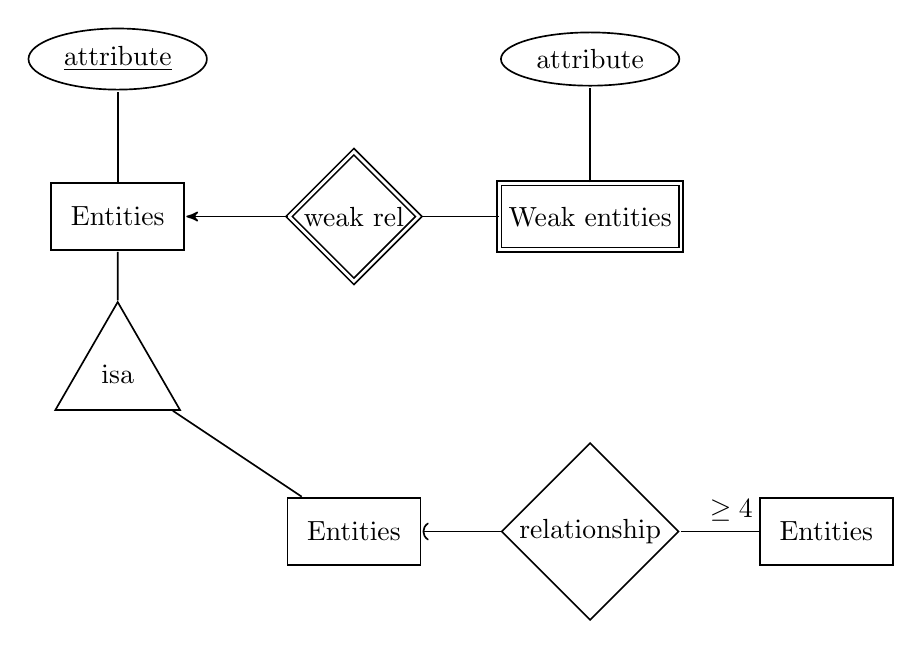
\begin{tikzpicture}[>=stealth', semithick,                                                  % More pronounced edges
                        shorten >= 0.5, node distance = 2cm and 3cm, on grid, auto,             % Node placement settings
                        isa/.style = {regular polygon, regular polygon sides=3, draw=black}]    % Defining isa nodes
        \node[entity] (ent1) {Entities};
        \node[attribute] (attr1) [above =of ent1] {\underline{attribute}};
        \node[relationship, double distance=0.1em] (wrel) [right =of ent1] {weak rel};
        \node[entity, double distance=0.1em] (went) [right =of wrel] {Weak entities};
        \node[attribute] (attr2) [above =of went] {attribute};
        \node[isa] (isa) [below =of ent1] {isa};
        \node[entity] (ent2) [below right =of isa] {Entities};
        \node[relationship] (rel1) [right =of ent2] {relationship};
        \node[entity] (ent3) [right =of rel1] {Entities};
        %edge:many
        \path[-]
            (ent1) edge (attr1)
            (went) edge (wrel)
            (went) edge (attr2)
            (isa) edge (ent1)
            (isa) edge (ent2)
            (ent3) edge node [above, pos = 0.35] {$\geq 4$} (rel1);
        %edge:one
        \path[->]
            (wrel) edge (ent1);
        %edge:exactly-one
        \path[-)]
            (rel1) edge (ent2);
    \end{tikzpicture}
    \label{fig:ER}
\end{figure}

\section{Referencer} \label{sec:ref}
Skal man have en reference til ligninger, figurer, afsnit eller andet, så bruges \emph{ref} kommandoen. Et \emph{ref} vil altid pege på et \emph{label}. For eksempel er dette afsnit nummer \ref{sec:ref}. I afsnit \ref{sec:math} er der en ligning \ref{eq:alignatL2}

Vil man dog lave en reference til litteraturlisten, så bruges \emph{cite} kommandoerne. Her er desuden en reference til litteratur \cite{bibEks}, som er skrevet i \emph{bibliography} længere nedenunder. Dette er dog redefineret til litteratur i danskdelen ovenfor. Vil man have flere referencer samtidig, så skrives bare flere referencer som argumenter til \emph{cite}, så det ser sådan ud: \cite{bibEks, steffan}

\section{Citater}
Med \emph{csquotes} pakken er det muligt at lave pæne citater, såsom Steffan's udsagn \textcquote[s. 12]{steffan}{Vi er dataloger, ikke vampyrer.}. Ved brug af \emph{blockquote} fås automatisk et fremhævet citat, sålænge det er 4+ linjer.

\blockcquote[s. 1]{bibEks}{Lorem ipsum dolor sit amet, consectetur adipiscing elit, sed do eiusmod tempor incididunt ut labore et dolore magna aliqua. Ut enim ad minim veniam, quis nostrud exercitation ullamco laboris nisi ut aliquip ex ea commodo consequat. Duis aute irure dolor in reprehenderit in voluptate velit esse cillum dolore eu fugiat nulla pariatur.}

Bemærk, at begge citater bruger et \emph{c} som prefix til \emph{quote}. Dette giver muligheden for at referere til litteraturlisten. Hvis dette ikke ønskes, så kan man fjerne \emph{c} og fjerne referencer samtidig.

\newpage
\section{Kolonner}
\begin{multicols}{2}

\noindent Her er tekst opdelt i to kolonner, hvilket kan bruges til mange ting. Måske have et billede til venstre eller kode? Hvis du vil bruge kode, skal du dog fjerne header og centering indstillingerne øverst.

\vfill \columnbreak

Her er noget tekst i den anden kolonne. Dette kunne også bruges til at have titel og abstract til venstre og indholsfortegnelse til højre?

\end{multicols}

\begin{thebibliography}{9}
\bibitem{bibEks}
 Efternavn, Fornavn: \emph{Artikel titel}, 20xx
\bibitem{rasmus}
 Skovdal, Rasmus: \emph{Calculus 1}, 2015
\bibitem{steffan}
 Jørgensen, Steffan: \emph{101 citater}, 2015

\bibitem{referencer.bib}
 Man kan enten skrive litteraturen i sit dokument, eller have en ekstra referencer.bib fil med al information:

@book{FilVri97,
Author = {Filar, Jerzy and Vrieze, Koos},
Publisher = {Springer},
Title = {Competitive Markov Decision Processes},
Year = 1997
} 
 
\end{thebibliography}
\bibliographystyle{abbrv}
\bibliography{referencer}

\newpage
\appendix
\section{Et Appendix}
Lorem ipsum dolor sit amet, consectetur adipiscing elit, sed do eiusmod tempor incididunt ut labore et dolore magna aliqua. Ut enim ad minim veniam, quis nostrud exercitation ullamco laboris nisi ut aliquip ex ea commodo consequat.

\end{document}